\section{Evaluation Metrics}

The two main measurements for the performance of our new architecture are learning efficiency and transfer learning capability.
The learning efficiencies are measured in two different ways. First, the algorithm performance is compared with exisitng RL algorithms in terms of
convergence rate, which is measured in terms of number of episodes that the agent needs to get to an optimal policy.
Second, ILASP learning is measured in each episodes and time steps to see how the new algorithm refines its internal hypothesis over time.
Other common measurements in RL are XXX, XXX, but our primary goal of this research is data-efficient learning.

% We use GVG-AI Framework for our experiments, which was created for the General Video Gamea AI Competition\footnote{http://www.gvgai.net/},
% a game environment for an agent that should be able to play a wide variety of games without knowing which games are to be played.
\subsection{Experiment Platform}
We use the Video Game Definition Language (VGDL), which is a high-level description language for 2D video games providing a platform for computational intelligence research (\cite{Schaul2013}).
The VGDL allows users to easily craft their own environments, which makes us possible to do various experiments without relying on a default environment. The VGDL platform provides an interface with OpenAI Gym (\cite{Brockman2016}), which is a commonly used benchmark platform. 
The base game is a simple maze as shown in Figure \ref{VGDL_sample}.
There are 3 different types of cells: a goal cell, walls and paths. The agent can take 4 different actions: up, down, right and left.
The environment is not known to the agent in advance, and it attempts to find the goal by exploring the environment.

\begin{figure}[!ht!b]
    \centering
    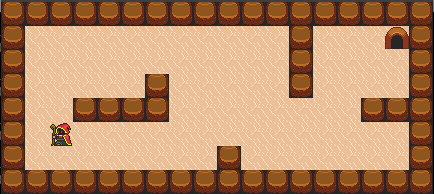
\includegraphics[width=0.5\textwidth]{./figures/experiment1}
    \caption{VGDL game example}
    \label{VGDL_sample}
    \end{figure}    
\subsection{Benchmark}
We use two existing reinforcement learning methods as benchmarks: Q-learning and tile-coding. 
Q-learning is most widely used technique for reinforcement learning. Given our environment is deterministic and discrete, this method works well in our environment.
Another benchmark is tile coding, which is a type of linear function approximation techniques described in Chapter XX.
The reason for using another extra benchmark is that the comparision with q-learning might not be a fair comparision,
since our algorithm has one extra assumptions: the agent knows surrounding information (whether there are walls in adjacent cells),
which is not a common assumption for Q-learning. Thus we incorporate the same surrounding information as features, and update the weights of each feature as a learning.
We compare the performance of our algorithm with these two methods.

\subsection{Parameters}
In all experiments, the agent receives -1 in any states except the goal state, where it gains a reward of 10.
All the matrices used in the experiments are summarised in Table \ref{param}. 

\begin{table}[!ht!b]
\centering
\begin{tabular}{lll}
\hline
Parameter            & My algorithm    & Benchmark      \\ \hline
The number of episode& 100        & 100        \\
Time step per episode& 250        & 250        \\
The number of experiments& 30       & 30       \\
% Discount rate        & 0,5       & 1.4e-2       \\
Alpha                & N/A       & 0.5       \\
Epsilon              & 0.4        & 0.1        \\
\end{tabular}
\caption{Parameters of the initial and optimised fully connected network.}
\label{param}
\end{table}

Epsilon for our algorithm should be higher, since the agent follows the generated plan, 
whereas benchmark algorithms update value function with the degree of alpha. 
We conducted several experiments using different environments to highlight each aspect of the algorithm.

\section{Experiment Results}
\label{learning_evaluation}

\subsection{Experiment1}
The purpose of the first experiment is how the algorithm learns the model of the environment, or hypothesis in ILASP.

\begin{figure}[!htb]
\centering
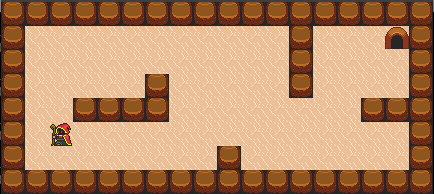
\includegraphics[width=0.5\textwidth]{./figures/experiment1}
\caption{Enviroment for experiment 1}
\label{experiment1}
\end{figure}

\begin{figure}[!htb]
\centering
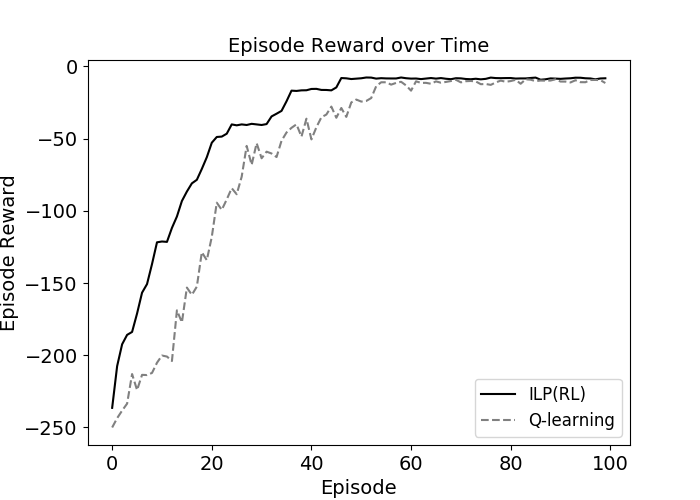
\includegraphics[width=1.0\textwidth]{./figures/experiment1_training}
\caption{Comparison of training performance between my algorithm and Q-learning}
\label{experiment1_training}
\end{figure}

\begin{figure}[!htb]
\centering
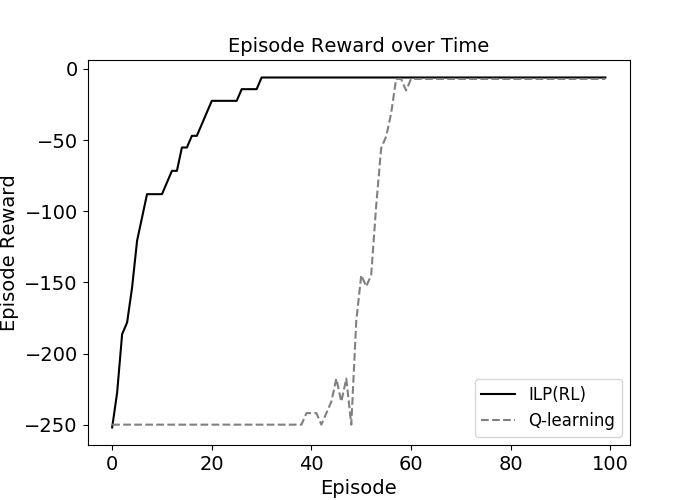
\includegraphics[width=1.0\textwidth]{./figures/experiment1_test}
\caption{Comparison of test performance between my algorithm and Q-learning}
\label{experiment1_test}
\end{figure}

\begin{figure}[!htb]
\centering
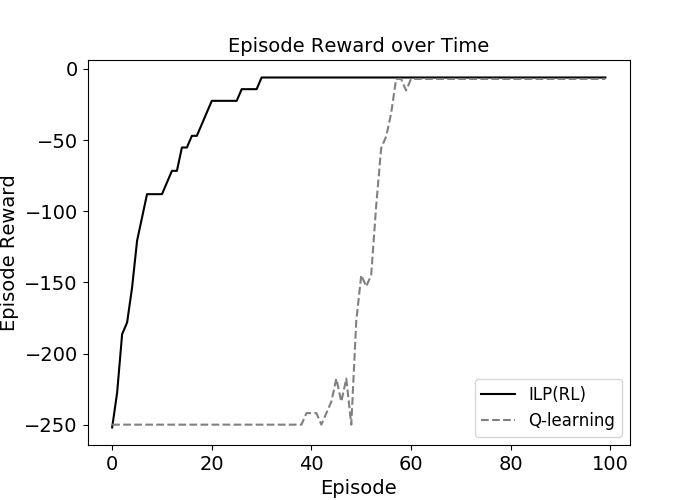
\includegraphics[width=1.0\textwidth]{./figures/experiment1_test}
\caption{PLACEHOLDER FOR ILASP}
\label{experiment1_test}
\end{figure}

Learnt hypotheses are as follow:
\begin{equation*}
\begin{split}
&\textsf{state\_after(V1) :- adjacent(right, V0, V1), state\_before(V1), action(right), wall(V0).}\\
&\textsf{state\_after(V0) :- adjacent(right, V0, V1), state\_before(V0), action(left), wall(V1).}\\
&\textsf{state\_after(V1) :- adjacent(down, V0, V1), state\_before(V1), action(down), wall(V0).}\\
&\textsf{state\_after(V1) :- adjacent(up, V0, V1), state\_before(V1), action(up), wall(V0).}\\
&\textsf{state\_after(V0) :- adjacent(right, V0, V1), state\_before(V1), action(right), not wall(V0).}\\
&\textsf{state\_after(V0) :- adjacent(left, V0, V1), state\_before(V1), action(left), not wall(V0).}\\
&\textsf{state\_after(V0) :- adjacent(down, V0, V1), state\_before(V1), action(down), not wall(V0).}\\
&\textsf{state\_after(V0) :- adjacent(up, V0, V1), state\_before(V1), action(up), not wall(V0).}
\end{split}
\end{equation*}

% Converge to optimal policy faster than Q-learning.

\subsection{Experiment2}

TODO Comparison with Tile Coding
% The first experiment might not be a fair comparision between our algorithm and Q-learning, since our algorithm has extra information about the surrounding information.
% In order to have the same assumptions, we use function approximation for Q-learning.
% Linear function approximation.
% \begin{figure}[!htb]
% \centering
% 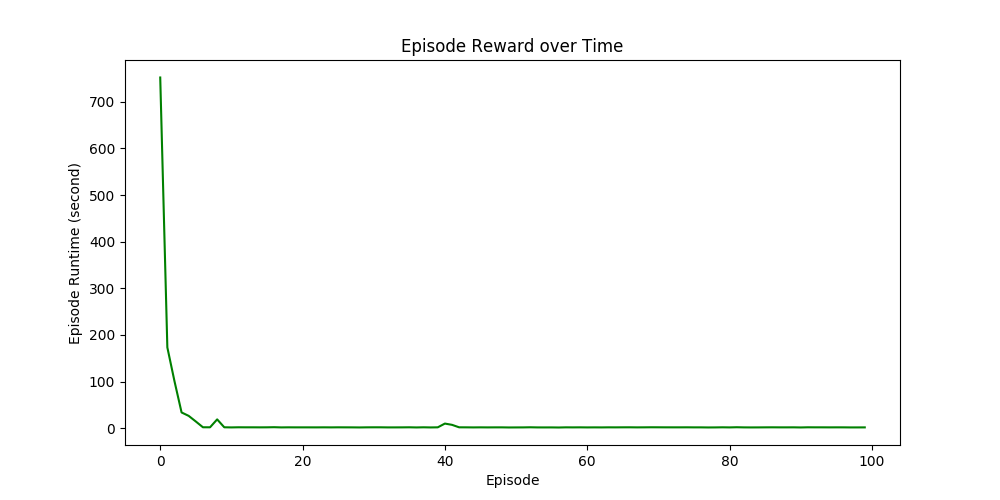
\includegraphics[width=1.0\textwidth]{./figures/placeholder}
% % 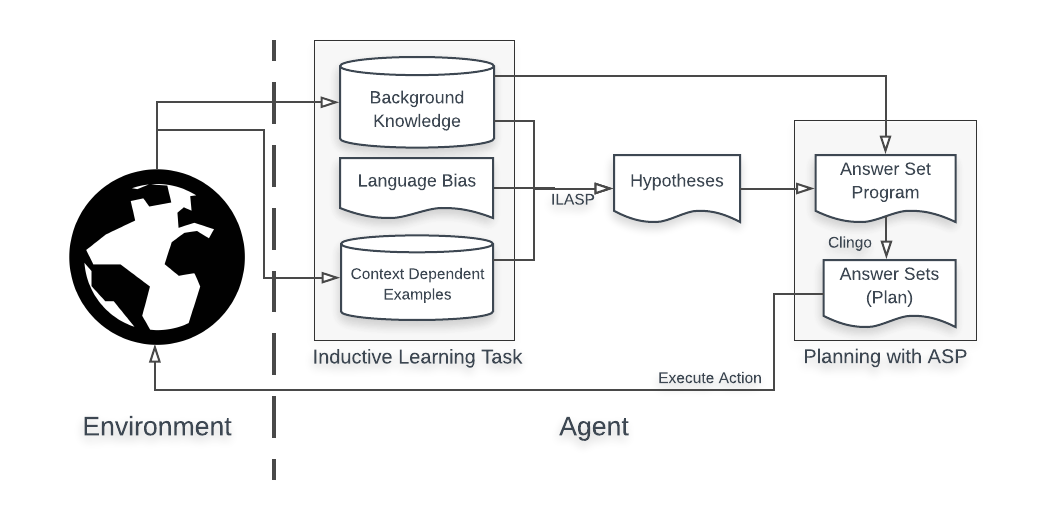
\includegraphics[width=10cm, height=9cm]{./figures/architecture}
% \caption{PLACEHOLDER}
% \label{proposed_architecture}
% \end{figure}
\newpage
\subsection{Experiment3}
% The game is designed such that

\begin{figure}[!htb]
\centering
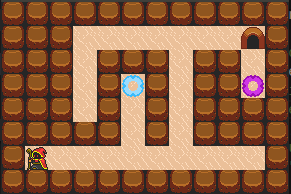
\includegraphics[width=0.5\textwidth]{./figures/experiment3_v2}
\caption{Enviroment for experiment 3}
\label{experiment3}
\end{figure}

This experiment is conducted to see if the agent find a optimal path of using a teleport.

\begin{figure}[!htb]
\centering
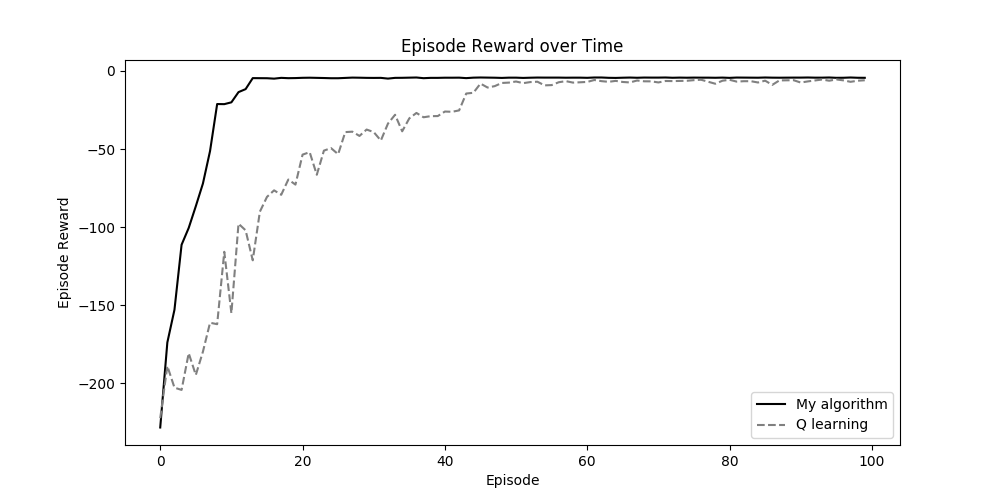
\includegraphics[width=1.0\textwidth]{./figures/experiment3_training}
\caption{Comparison of training performance between my algorithm and Q-learning}
\label{experiment3_training}
\end{figure}

\begin{figure}[!htb]
\centering
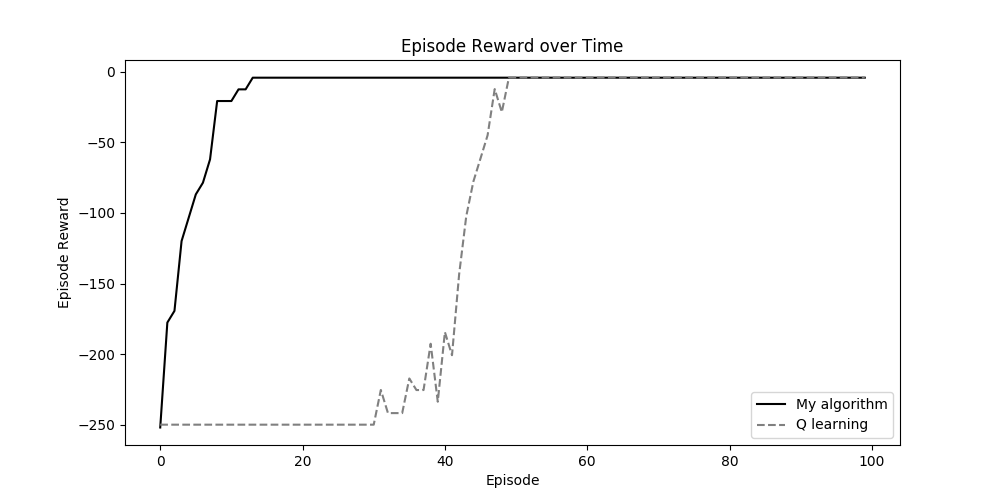
\includegraphics[width=1.0\textwidth]{./figures/experiment3_test}
\caption{Comparison of test performance between my algorithm and Q-learning}
\label{experiment3_test}
\end{figure}

\begin{figure}[!htb]
\centering
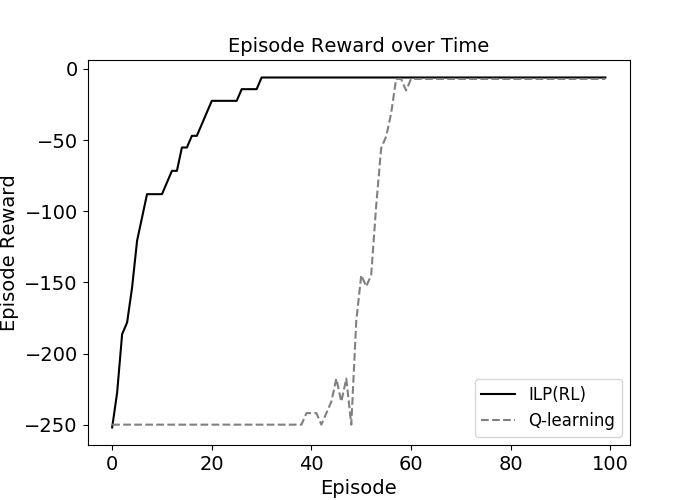
\includegraphics[width=1.0\textwidth]{./figures/experiment1_test}
\caption{PLACEHOLDER FOR ILASP}
\label{experiment1_test}
\end{figure}

Learnt hypotheses are as follow:
\begin{equation*}
\begin{split}
&\textsf{state\_after(V1) :- link\_start(V0), link\_dest(V1), state\_before(V0).}\\
&\textsf{state\_after(V0) :- link\_dest(V0), state\_before(V0), action(right).}\\
&\textsf{state\_after(V1) :- adjacent(left, V0, V1), state\_before(V0), action(right), not wall(V1).}\\
&\textsf{state\_after(V0) :- adjacent(left, V0, V1), state\_before(V1), action(left), not wall(V0).}\\
&\textsf{state\_after(V1) :- adjacent(up, V0, V1), state\_before(V0), action(down), not wall(V1).}\\
&\textsf{state\_after(V0) :- adjacent(up, V0, V1), state\_before(V1), action(up), not wall(V0).}\\
&\textsf{state\_after(V1) :- adjacent(left, V0, V1), state\_before(V1), action(left), wall(V0).}\\
&\textsf{state\_after(V1) :- adjacent(down, V0, V1), state\_before(V1), action(down), wall(V0).}\\
&\textsf{state\_after(V1) :- adjacent(up, V0, V1), state\_before(V1), action(up), wall(V0).}
\end{split}
\end{equation*}

\newpage
% \section{Transfer Learning Evaluation}
% \label{transfer_learning}

\subsection{Experiment4}

\begin{figure}[!htb]
\centerline{
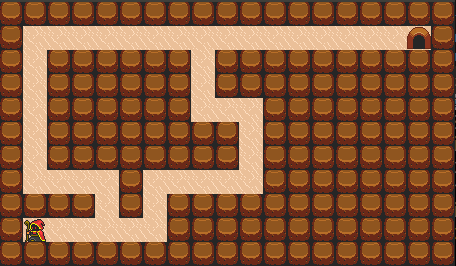
\includegraphics[width=0.5\textwidth]{./figures/experiment4_before}
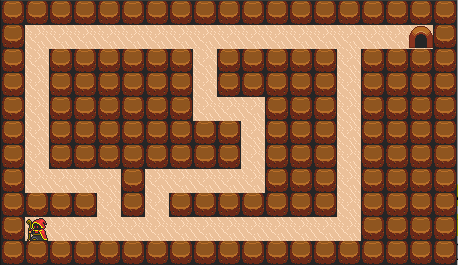
\includegraphics[width=0.5\textwidth]{./figures/experiment4_after}
}
\caption{Before (left) and after (right) transfer learning}
\label{experiment4}
\end{figure}

Finally, we investigated the potentials of transfer learning betweeen similar environments.

The goal position is the same as in the first game, but the routes to the goal are different.

% Experiment 4 Transfer learning
%     1 update B
%     2 update H

% \textsf{\#modeb(1, link(var(cell), var(cell)), (positive)).}
\begin{figure}[!htb]
\centering
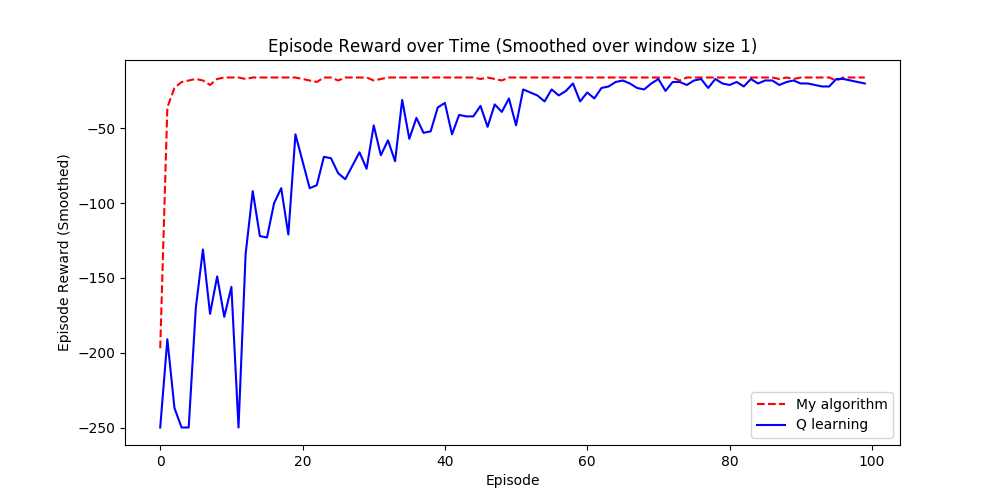
\includegraphics[width=1.0\textwidth]{./figures/experiment4_before_training}
\caption{Comparison of training performance between my algorithm and Q-learning (before transfer)}
\label{experiment3_training}
\end{figure}

\begin{figure}[!htb]
\centering
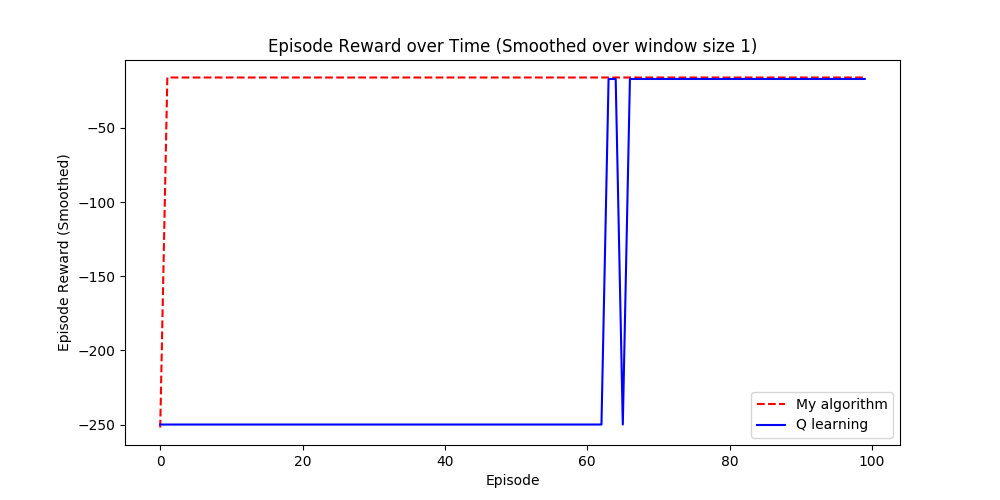
\includegraphics[width=1.0\textwidth]{./figures/experiment4_before_test}
\caption{Comparison of test performance between my algorithm and Q-learning (before transfer)}
\label{experiment3_test}
\end{figure}

\begin{figure}[!htb]
\centering
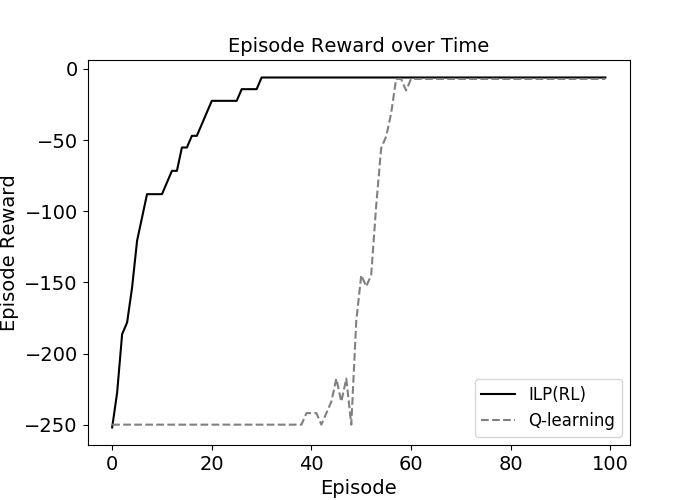
\includegraphics[width=1.0\textwidth]{./figures/experiment1_test}
\caption{PLACEHOLDER FOR ILASP}
\label{experiment1_test}
\end{figure}


These are the hypotheses we are transferring to a new environment.
\begin{equation*}
\begin{split}
 &\textsf{state\_after(V0) :- adjacent(right, V0, V1), state\_before(V1), action(right), not wall(V0).}\\
 &\textsf{state\_after(V0) :- adjacent(left, V0, V1), state\_before(V1), action(left), not wall(V0).}\\
 &\textsf{state\_after(V1) :- adjacent(down, V0, V1), state\_before(V0), action(up), not wall(V1).}\\
 &\textsf{state\_after(V0) :- adjacent(down, V0, V1), state\_before(V1), action(down), not wall(V0).}\\
 &\textsf{state\_after(V1) :- adjacent(right, V0, V1), state\_before(V1), action(right), wall(V0).}\\
 &\textsf{state\_after(V1) :- adjacent(left, V0, V1), state\_before(V1), action(left), wall(V0).}\\
 &\textsf{state\_after(V0) :- adjacent(up, V0, V1), state\_before(V0), action(down), wall(V1).}\\
 &\textsf{state\_after(V1) :- adjacent(up, V0, V1), state\_before(V1), action(up), wall(V0).}
\end{split}
\end{equation*}

\subsubsection{Transfer learning}
\begin{figure}[!htb]
\centering
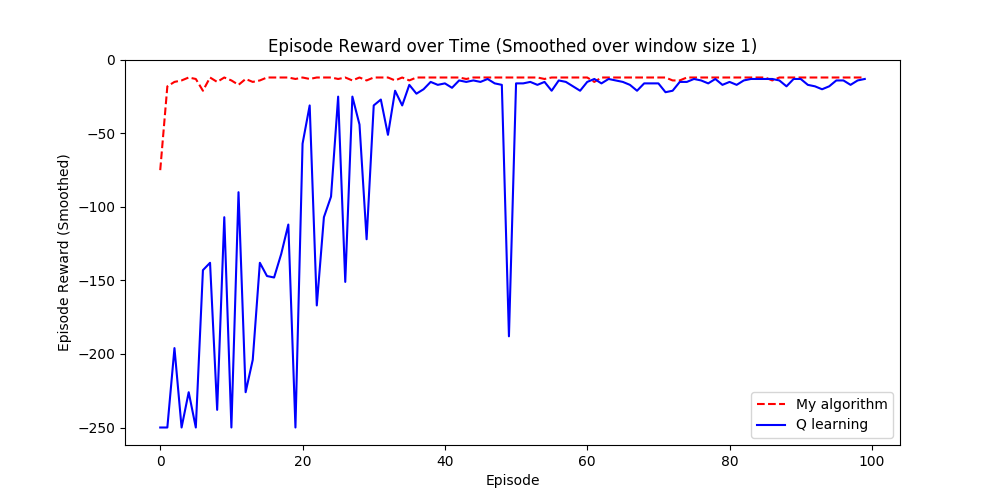
\includegraphics[width=1.0\textwidth]{./figures/experiment4_after_training}
\caption{Comparison of training performance between my algorithm and Q-learning (after transfer)}
\label{experiment3_training}
\end{figure}

\begin{figure}[!htb]
\centering
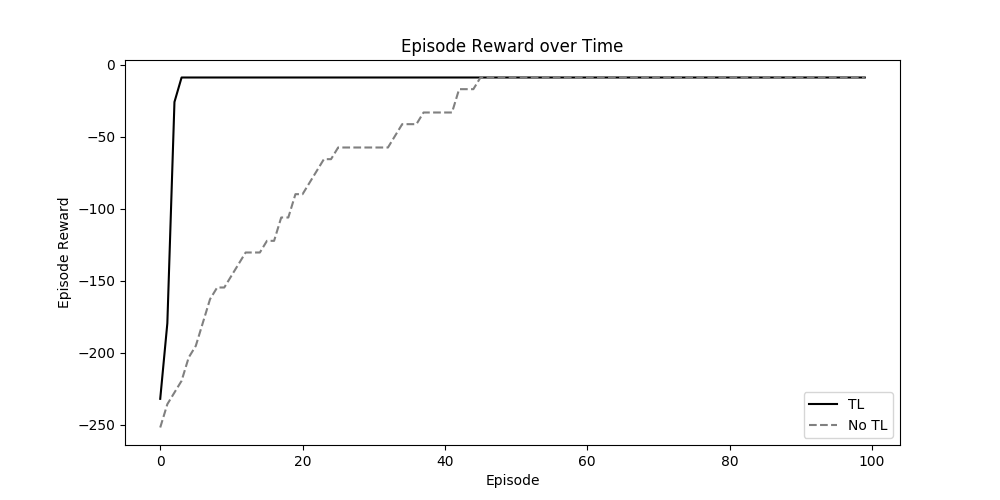
\includegraphics[width=1.0\textwidth]{./figures/experiment4_after_test}
\caption{Comparison of test performance between my algorithm and Q-learning (after transfer)}
\label{experiment3_test}
\end{figure}

These are the hypotheses we are transferring to a new environment.
\begin{equation*}
\begin{split}
\end{split}
\end{equation*}

\newpage
\subsection{Experiment5}

TODO Transfer learning for new H

% \subsection{Results}

% \subsection{Discussion}
% \subsubsection{Strengths}

% \subsection{Limitations}

% You have to define the search space for H

% Learning ILASP is known to be less scalable.

% ILASP learning is quite slow

% Another limitation is training time. Unlike existing reinforcement learning,
% out algorithm refines hypothesis at every time steps within the same episode.
% Thus even though the efficiency in terms of the number of iteration is higher,
% training time within each iteration tends to be lower.
% As stated in XXX
